This chapter is intended to recapitulate the background of the thesis theme. In
Sec.~\ref{sec:2.1}, we recall the evolution of software systems with respect to
architecture and variability. In Sec.~\ref{sec:2.2} we outline the characteristics
of software performance, practical testing and measurement strategies as well as
some statistical background necessary to analyze, interpret and compare
performance assessment. In Sec.~\ref{sec:2.3} we present recent approaches for
feature model extraction from existing software systems and code artifacts. Finally, in
Sec.~\ref{sec:2.4} we recall and compare in detail different approaches to model
and predict performance behavior for configurable software systems.




\section{Evolving Software} \label{sec:2.1}
\paragraph{Software Evolution}
The first notion of a software systems' development process is usually
developer-centered and merely focuses on software being designed, implemented,
tested and eventually being released and deployed. Maintainability is a
generally recognized software quality property to look after, and maintenance
is, of course, essential to every successful software system. Nonetheless, less
attention is given to the ability to adapt a software system to changing
requirements (evolvability) rather than maintaining it to keep functionality
working \citep{parnas_software_1994}. Software evolution and evolvability, like
software itself are manifold. Software evolves in many ways ranging from maintenance (refactoring,
bug-fixes and patches) to adapting to changed requirements (adding, removing,
reorganizing functionality and variability).

Modern software systems not only often ship with a variety of configuration
options to select, they also employ routines to be build and sometimes even
make use of or are part of platforms, such as apps or plugins. That is,
software evolution affects all aforementioned aspects and maintainability as
well as evolvability can degrade as software evolves.

\paragraph*{Software Erosion}
The negative symptoms of software evolution, which are referred to as
``architectural erosion'' \citep{breivold_systematic_2012}, have
been addressed by many researchers.
Most of existing research so far though focuses on evolution regarding software architecture
\citep{breivold_systematic_2012}. The main driving factors leading to symptoms of decay
identified by \cite{perry_software_1991} are architectural erosion and
architectural drift. While architectural drift subsumes developers'
insensitivity when not following a systems architecture or respective guidelines while making changes, architectural erosion subsumes ignoring and violating the existing software
architecture. \cite{parnas_software_1994} argues that as software evolves, software is maintained
and evolved by developers who are not necessarily familiar with the initial
architectural design and, therefore, knowledge about the architecture becomes
unavailable. Although the unfavorable effects of software evolution do not necessary break a
system necessarily and imminently, the software becomes ``brittle'' \citep{perry_software_1991}
as maintainability as well as evolvability degrade. Concrete  symptoms of software
erosion on the implementation level have been documented. 

\cite{zhang_variability_2013} have studied erosion symptoms for a large-scale
industrial software product line with compile-time variability using
preprocessor directives.
They identify variability-related directives and clusters of those to tend to become more
complex as the software evolves. The negative effects, or symptoms of software
erosion are described as, but not limited to \emph{code replication} or
interdependencies between code elements, such as \emph{scattering} and
\emph{tangling}. Code scattering describes the phenomenon of code belonging to
a certain feature being scattered across multiple units of implementation,
e.g., modules, whereas code tangling means that code from different and
potentially unrelated features in entangled within a single module.

\cite{passos_feature_2015} have studied the extent of usage of scattering for device-drivers
in the Linux kernel. Despite scattering being quite prevalent, their
findings suggest that the kernel architecture is robust enough to have evolved
successfully. Nonetheless, platform drivers in the Linux kernel seem more
likely to be scattered than non-platform driver. They conclude that this is a
trade-off between maintainability and performance: a more generalized and
abstract implementation for platform-drivers in this case could possibly avoid
scattering, yet refactorings in this manner did not seem to be necessary or
worth the effort yet.

\paragraph*{Variability Evolution}
Apart from architecture evolution, the variability offered by software systems
evolves as well. For configurable software systems (or software product lines; 
these terms are not equivalent, but every SPL is a configurable software system)
evolution steps will not only affect artifacts in the solution space, yet also be visible in changes in the respective variability models.
Although the variability aspect of software evolution has not been drawn as
much attention to as has been on architecture in the past, more and more
research has emerged recently to address and understand variability evolution.

\cite{peng_analyzing_2011} proposed a classification of variability evolution patterns that
conceives evolution as adaption to changing (non-)functional requirements as
well as changing contexts. For a context in that sense, two
categories exist. A driving context determines, whether a variability model and respective variants
can meet functional requirements in the first place. A supporting context by
definition determines how non-functional properties are strengthened or
weakened. Any changed requirement is likely to change the contexts for a
software systems variability model and, therefore, will make adaptations of the
variability model necessary. Within their classification method Peng et al.
identify  major causes for variability evolution, comprising a) new driving
contexts emerging, b) weakened supporting contexts (for instance, due to new
non-functional requirements), and c) unfavorable trade-offs for non-functional
properties. 

To understand single evolutionary steps, several catalogs of variability
evolution patterns have been proposed. \cite{peng_analyzing_2011} present three patterns,
where either a new feature is added, a mandatory feature becomes optional, or a
mandatory/optional feature is split into alternative features. \cite{seidl_co-evolution_2012} suggest a catalog of
patterns for co-evolution of variability models and feature mappings that additionally introduces code clones, splitting a feature
into more fine-grained sub-features and feature removal as evolution patterns.
In addition, \cite{passos_towards_2012} have studied variability evolution in
the Linux kernel and present a catalog of patterns where features are removed from the
variability model, but remain a part of the implementation. Their
catalog, among others, includes feature merges, either implicit (optional feature merged
with its parent) or explicit.

The classification proposed by \cite{peng_analyzing_2011} is a general and formalized approach
that, as well as \cite{seidl_co-evolution_2012} and \cite{passos_towards_2012}, describes
elementary evolution patterns which can be composed to more complex patterns. Nonetheless, no
comprehensive catalog of variability evolution so far has been proposed as all
mentioned work above focuses on those patterns that appeared to be relevant for
the respective case study.

\section{Variability Modeling}
{\color{violet}
The design and development of configurable software systems is conceptually
divided into \emph{problem space} and \emph{solution space} \citep{czarnecki_generative_2000}. The problem space
comprises the abstract design of features that are contained in the software system as well as
constraints among features, such as dependencies or mutual-exclusion. The
solution space describes the technical realization of features and the
functionality described by and associated with features, e.g., implementation
and build mechanisms. That is, features cross both spaces since they are mapped
to corresponding code artifacts.

A common way to express features and constraints in the problem space is to
define a \emph{variability model}, or \emph{feature model}, which subsumes all
valid configurations
\citep{kang_feature-oriented_1990,apel_feature-oriented_2013}. There are different and equivalent syntactical approaches to define feature models, for instance, a propositional formula $F$ over the set of
features of the configurable software systems \citep{batory_feature_2005}. In
this case a configuration is valid with respect to the feature model if and only if $F$ holds for all
selected features being true and all unselected features being false respectively. 
However, a more practical and more commonly used way to express feature models
are graphical tree-like \emph{feature diagrams}
\citep{apel_feature-oriented_2013}. In a feature diagram, features are ordered
hierarchically, starting with a root feature and subsequent child features. By
definition, the selection of a child feature requires the parent feature to be
selected as well. Child features can either be labeled as \emph{optional}
features  or \emph{mandatory} features; the latter ones need to be selected in
every valid configuration.
Moreover, feature diagrams
provide a syntax for two different types of feature groups, \emph{or-groups} or
\emph{alternative-groups}. For an or-group at least one of the group's features
needs to be selected for a valid configuration, whereas for an alternative group
exactly one out of the group's mutually exclusive features must be selected. In
addition to the feature hierarchy, constraints, which cannot be expressed by
the tree-like structure, are referred to as \emph{cross-tree constraints}.
Cross-tree constraints, depending on the notation, are depicted by arrows
between two features or simply added to the feature diagram as a propositional
formula. For such two features $f_1$ and $f_2$, a cross-tree constraint means
that for feature $f_1$ to be selected, either the selection of $f_2$ is
required/implied or excluded.

An introductory example for the syntax and semantics of feature diagrams is
provided in Fig.~\ref{fig:introduction_fm}. In this example an imaginary
vehicle propulsion can be configured with eight valid configurations. The vehicle requires an engine,
thus, feature \textsf{Engine} is mandatory. At least one out of the three
features \textsf{Hybrid}, \textsf{Piston} and \textsf{Electric} needs to be
selected. For a piston engine, we can select either the feature \textsf{Diesel}
or \textsf{Petrol}. A petrol engine requires additional ignition sparks in
contrast to a Diesel engine. For an electric engine we require a
battery, hence, the feature \textsf{Battery} is mandatory.
In addition, the feature model specifies two cross-tree constraints: First, the
feature \textsf{Tank} is optional, yet once a piston engine is selected, we
require  a tank. Second, if we want to use the \textsf{Hybrid} functionality
(e.g., use both electric and piston engine simultaneously), we require to have both a piston
and an electric engine.

\begin{figure}[htbp]
  \centering
  
  	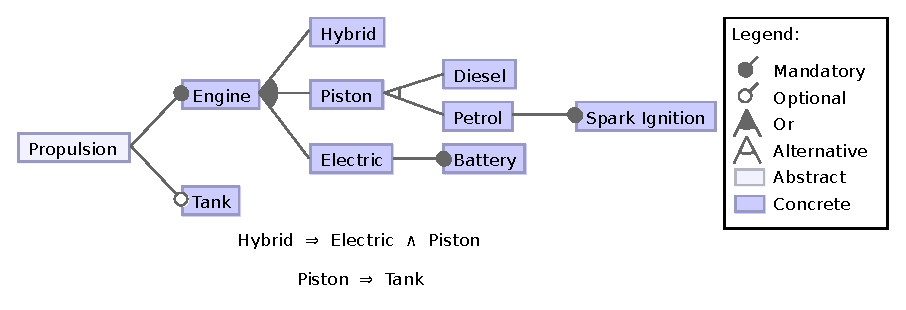
\includegraphics[width=0.85\textwidth]{images/introduction_fm.eps}
  \caption{Feature diagram for a feature model with eight valid configurations;
  two cross-tree constraints are specified as propositional formulas over
  features}
  \label{fig:introduction_fm}
\end{figure}}

\section{Feature Model Synthesis}  \label{sec:2.3}
A variability model as an abstraction of functionality of a software system is
required, or at least of great interest, in many contexts. \emph{First}, not
every configurable system (or software product line) provides an explicit
representation of its variability model. 
The reasons for inexplicit or absent configuration specification are manifold.
They can range from poor or inconsistent documentation
\citep{rabkin_static_2011}, overly complex configurability \citep{xu_hey_2015}
or configuration constraints originated in different layers of a software
system, e.g.m build constraints  or compiler constraints \citep{nadi_where_2015}. 

\emph{Second}, variability models have emerged to be a useful means in domain
and domain analysis prior to developing a software system. As variability
models group and organize functionality, synthesizing a variability model has
shown to be applicable to extract features and constraints from functional
requirements. In addition, by comparison of product specifications for an
existing market domain, variability models can provide detailed feature summary.

For this thesis, we focus on the first aspect of synthesizing variability
models, as our work addresses the assessment of already existing configurable
software systems. Nonetheless, many techniques employed in the aforementioned
second aspect address similar problems, yet rely on natural language artifacts
rather than code artifacts \citep{alves_exploratory_2008,bakar_feature_2015}.
The following section recalls work on extracting configuration options and
constraints from source code as well as the organization of constraints into
feature hierarchy and groups. The further assessment of configurable systems
requires a well-defined and sound variability model.

\subsection{Feature Extraction} 
The first objective in recovering a variability model from a configurable
system is to determine the set of available configuration options to select. In
addition, for further configuration the type of each configuration option
(e.g., boolean, numeric or string) and the respective domain of valid values
needs to be specified.

\cite{rabkin_static_2011} proposed a static, yet heuristic approach to extract
configuration options along with respective types and domains. They exploit the
usage of configuration APIs. Their approach works
in two stages and commences with extracting all code sections where
configuration options are parsed. Subsequently, configuration names can be
recovered as they are either already specified at compile-time or can be
reconstructed using string analysis yielding respective regular expressions.
Moreover, they employ a number of heuristics to infer the type of parsed
configurations as well as respective domains. First, the return type of the
parsing method is likely to indicate the type of the configuration option read.
Second, if a string is read initially, the library method it is passed to can
reveal information about the actual type. For instance, a method
\emph{parseInteger} is likely to parse an integer value. Third, whenever a
parsed configuration option is compared against a constant, expression or value of an enum class,
these might indicate valid values or at least corner cases of the configuration
options' domain. The extraction method by \cite{rabkin_static_2011} renders to be precise, but is
limited, for instance, when an option leaves the scope of the source code.
Nonetheless, for the systems they evaluated they recovered configuration
options that were not documented, only used for debugging or even not used at
all.

\subsection{Constraint Extraction}
The second, or an additional step in recovering a variability model is the
extraction of configuration constraints. An approach proposed by \cite{zhou_extracting_2015}
focuses on the extraction of file presence conditions from build files using symbolic execution. A more comprehensive investigation of configuration
constraints and their origin is provided by \cite{nadi_mining_2014,nadi_where_2015}. They
propose an approach based on variability-aware parsing and infer constraints by
evaluating make files and  analyzing preprocessor directives. Inferred
constraints result from violations of two assumed rules, where a) every valid
configuration must not contain build-time errors and b) every valid
configuration should result in a lexically different program, thus. While the
first rule aims at inferring constraints that prevent build-time errors, the
second one is intended to detect features without any effect, at least as part
of some configurations. Their analysis one the one hand emerged to be accurate
in recovering constraints with 93~\% for constraints inferred by the first rule
and 77~\% for second one respectively. On the other hand, their approach was
only to recover 28~\% of all constraints present in the software system.
Further qualitative investigation, including developer interviews, lead to
the conclusion that most of existing constraints stem from domain knowledge.

\subsection{Reverse Engineering of Feature Hierarchy} 
Besides recovering configuration options and respective constraints, to reverse
engineer a feature model, one further step is required. The recovered knowledge
needs a tree-like hierarchy, detection of feature groups and cross-tree
constraints to be an acceptable feature diagram
\citep{kang_feature-oriented_1990}. While several approaches to the recover feature model hierarchy have been proposed,
we are primarily interested in finding a hierarchy for knowledge obtained from
source code. Other scenarios, as already stated in the opener of this section,
are based on product descriptions or sets of valid configurations. The remainder of
this subsection we will focus on organizing features and constraints extracted
from source code. For further reading \cite{andersen_efficient_2012} present algorithms
for structuring feature diagrams for three different scenarios including the
ones previously mentioned.

Given an extracted set of features along with corresponding descriptions and
recovered constraints among the features, \cite{she_reverse_2011} propose an
semi-automated and interactive approach to synthesize a feature hierarchy.
Their approach comprises three steps: 1) Specifying a feature hierarchy, 2)
detecting and selecting feature groups, and 3) adding a cross-tree constraint
formula to the feature  model.

\begin{enumerate}
  \item Their approach commences with finding a single parent for each
  feature and, thus, specifying a tree-like feature hierarchy. Based on the
  given constraints a directed acyclic graph (DAG) representing implication
  relationships among features, a so-called implication graph, is constructed:
  Every vertex depicts a feature and edges are inserted for each pair of
  features $(u, v)$, where  $u \implies v$ holds with respect to the given
  constraints.
   
  In addition to the implication graph, the algorithm for each feature computes
  two rankings of features that are likely to be the respective parent feature.
  The two rankings both employ the feature descriptions. Feature descriptions
  are compared for similarity using a similarity metric. For two features $p$
  and $s$ the similarity is defined as the weighted sum of the inverse document
  frequencies $idf(w)$ for the words that the descriptions of features $u$ and
  $v$ share.
  The idf-ranking for a word $w$ is the logarithm of the number of features
  divided by the number of features whose description contains $w$. Each $idf$
  value is weighted by with by the frequency of $w$ in the description of
  feature $p$.
  
  The first ranking, called Ranked-Implied-Features (RIF), for each feature $f$
  ranks features by their similarity to $f$ in an descending order, but
  prioritizes those features that are implied according to the previously
  computed implication graph. The second ranking, called Ranked-All-Features
  (RAF) is similar to RIF, yet less strict since implied features are not
  prioritized. Given these ranking, a user selects for each feature a suitable
  parent feature from the RIF or RAF ranking. The idea behind providing two
  separate rankings, according to \cite{she_reverse_2011} is that the given
  extracted constraints can be incomplete and, thus, not all relevant implications are
  contained.

  \item After the feature hierarchy is specified, another auxiliary graph, a
  mutex graph, similar to the implication graph, is constructed. The mutex
  graph is an undirected graph with features as vertices and edges between two
  features $u$ and $v$, if $u \implies \neg{v}$ and $v \implies \neg{u}$ hold
  with respect to the given constraints. That is, all incident adjacent are mutually exclusive. Based on
  this mutex graph all maximal cliques (subsets of vertices that all are
  connected with each other) among the vertices with the same parent are
  computed. Those cliques are mutually exclusive and share the same parent and
  represent mutex- or alternative-groups. \cite{she_reverse_2011} introduce an
  additional constraint to extract xor-groups that require one of the groups’
  features to be selected if the parent is selected. This distinction is in
  line with the initial description of feature diagrams by \cite{kang_feature-oriented_1990},
  but not all descriptions follow this distinction between mutex- and
  xor-groups and just use the term alternative-group mentioned in Sec. 1.
  
  \item The cross-tree constraints for the feature diagram are extracted from
  the given configuration constraints. Since CTCs are constraints that could
  not be represented by the feature hierarchy (implication) or
  alternative-groups (exclusion) the derivation of CTCs follows this idea. The
  set of cross-tree implications is derived by removing all edges that are part
  of the feature hierarchy from the initially constructed implication graph.
  The set of cross-tree exclusions is derived in the same manner from the mutex
  graph by removing all edges among vertices of all mutex-groups. To make the
  feature model sound, the given configuration constraints, reduced to those
  clauses that are not already entailed by the diagram, can be added as an
  additional CTC formula to the feature diagram.
\end{enumerate}

The approach by \cite{she_reverse_2011} provides a practical algorithm to synthesize a
feature diagram, yet has some aspects we might need to consider. First, the
approach is not able to detect or-groups as defined in Sec. 1. Second, the
approach does introduce a root feature. Finally, the approach does not
distinguish between mandatory and optional features. Implicitly, all features
that do not have a parent feature are optional and all features that have a
parent feature are by default mandatory. \cite{she_reverse_2011} evaluated the
algorithm with both complete and incomplete variability knowledge (feature
names, descriptions and constraints). While the algorithm emerged to be
practical, detecting features whose parent was the root-feature was difficult.

\section{Performance Regression and Testing} \label{sec:2.2}
\begin{itemize}
  \item What is ``performance''? \citep{molyneaux_art_2014} 
  \item Ideas, concepts and strategies
  \citep{molyneaux_art_2014,fleming_how_1986,woodside_future_2007}
  \item Performance regression testing
  \citep{nguyen_industrial_2014,foo_mining_2010} and root cause detection
  \citep{heger_automated_2013}
\end{itemize}

\section{Performance Modeling} \label{sec:2.4}
\begin{itemize}
  \item Genetic algorithms \citep{guo_genetic_2011}
  \item Variability-aware modeling \citep{guo_variability-aware_2013}
  \item via feature-interaction and performance influence models
  \citep{siegmund_predicting_2012,siegmund_performance-influence_2015}
\end{itemize}